% To generate the summary
%\documentclass[english,10.5pt,letterpaper,twoside]{article}	% specify the class for style
%\usepackage{mathpazo}

\documentclass[english,11pt,letterpaper,twoside]{article}	% specify the class for style
\usepackage[T1]{fontenc}
\usepackage[latin9]{inputenc}
\usepackage{babel}
\usepackage{pslatex}		% use Adobe PostScript font (better than times)

% For URLs in the references
\usepackage{url}

% Advanced Math
\usepackage{amsmath}
\usepackage{amssymb}	% double line font letters (for number sets N,Z,D,Q,R)

% Images and Floats
\usepackage{epsfig}
%\usepackage{subfigure}
%\usepackage{lscape}			% landscape
%\usepackage{array}			% align vertically in tables
%\usepackage{multirow}

% Theorems, Definitions, ... (always after 'amsmath')
%\usepackage{amsthm}
%\theoremstyle{definition}
%\newtheorem{prop}{Proposition}%[section]
%\newtheorem{lemma}{Lemma}%[section]

% Algorithm environment
%\usepackage{algorithm}
%\usepackage{algorithmic}

% Commutative diagrams
%\usepackage{diagrams}


\usepackage[margin=1in]{geometry}
\setlength\headsep{20pt}

% Reduce the margins and spacings
\parskip 1mm

\frenchspacing	% no double space after end of line period.

% Add a header and footer
\usepackage{fancyhdr}
\pagestyle{fancy}
\fancyhead{}	% clear header
\fancyfoot{}	% clear footer (removes page number!)
% Set the header and footer content
%E: Even page
%O: Odd page
%L: Left field
%C: Center field
%R: Right field
%H: Header
%F: Footer
\usepackage{color}
\definecolor{light-gray}{RGB}{128,128,128}
\fancyhead[CO,CE]{\textit{\textcolor{light-gray}{\small Title}}}
\fancyfoot[LO,LE]{\textit{\textcolor{light-gray}{\small E. Syriani}}}
\rfoot{\thepage}
\renewcommand{\headrulewidth}{0.1pt}	% add a line with a specific thickness
\renewcommand{\footrulewidth}{0.1pt}	% add a line with a specific thickness
\newcommand{\monica}[1]{\textbf{\textcolor{red}{#1}}}
\newcommand{\eugene}[1]{\textbf{\textcolor{blue}{#1}}}

%%%%%%%%%%%%%%%%%%%%%%%%%%%%%%%%%%%%%%%%%%%%%

% Standard shortcuts
\newcommand{\eg}{\emph{e.g.,~}}							% exempli gratia (for the sake of example)
\newcommand{\ie}{\emph{i.e.,~}}							% id est (that is)
\newcommand{\etal}{~\emph{et al.}}					% et alia (and others)
\newcommand{\Fig}[1][Figure]{#1~}						% choose Fig. or Figure, depending on the style
\newcommand{\Sect}[1][Section]{#1~}					% section name always with a capital S
\newcommand{\Elem}[1]{\textsf{#1}}					% name of model element
\newcommand{\Lang}[1]{\textit{\textsf{#1}}}	% language, formalism name
\newcommand{\Rule}[1]{\texttt{#1}}					% rule name
\newcommand{\Code}[1]{\textit{\texttt{#1}}}	% inline code
\providecommand{\e}[1]{\ensuremath{\times 10^{#1}}}

%%%%%%%%%%%%%%%%%%%%%%%%%%%%%%%%%%%%%%%%%%%%%

\begin{document}
\fontsize{11.5}{13.5}\selectfont

%\normalem		% disables \emph to underline because overridden in ulem


\section*{\vspace{-2em}\center Project Summary}

Intelligent robots have not quite made it to the front lines of security and reconnaissance.  A more prevalent approach is to remotely tele-operate a robot from a safe distance to investigate and, if needed, disarm a threat.  However as research continues in intelligent algorithms, we expect that operators will become a peer of the robot, allowing for a higher robot to human ratio.  Unfortunately as algorithms become more intelligent, the practice of operators making in field hardware modifications to a robot will become an issue.  Updates to the hardware will need to be reflected in intelligent algorithms either autonomously or by highly-skilled operators.  

This proposal is about defining a specification that completely describes robot hardware devices in a way that enables three goals: 1) provide enough information for simulation and visualization of hardware and controllers, 2) declaratively specify the mechanism (both syntax and semantics) for requesting data and actuation, and 3) inform users of standard message types that can be obtained from the hardware to facilitate connection to existing frameworks.  RDIS (Robot Device Interface Specification) is a domain specific language that currently supports the syntax and semantics of differential drive robots and automates the creation of ROS drivers and command line programs.  We will expand RDIS to accommodate a larger set of kinematic designs, sensors and enabled tools and frameworks to move towards a specification that can be used to communicate hardware configuration changes to intelligent algorithms or operators. 

%\vspace{-.5\baselineskip}%
%\begin{itemize}
%	\item \textit{Challenge 1.}
%
%\vspace{-.5\baselineskip}%  
%	\item \textit{Challenge 2.}
%  
%\end{itemize}

\textbf{Intellectual Merit}

The intellectual merit of the proposed work centers on creating a domain-specific language to leverage the services provided on hardware devices by embedded firmware.  RDIS  provides a mechanism for centralizing the knowledge of the syntax (how to access the service) and semantics (what is the meaning of the input/output of the service) to the embedded system itself through a fully descriptive, declarative language.  This aspect of the proposed project is transformative: it could potentially affect the creation of new hardware platforms, reduce the complexity of device drivers (thus encourage new devices) and lower the learning curve to working with platforms.   To accomplish a specification that is generalizable, this project will expand a preliminary domain model that includes base concepts (linkages, joints and transmission) and account for simulation parameters (collision, appearance, dynamics, etc) to a more general set of popular platforms and kinematic linkages.  Although some frameworks use declarative specifications for hardware, none are complete or meet the needs of both simulation and capturing the interface syntax and semantics. It is expected that manufacturers will choose RDIS to enable their devices once there are more RDIS-enabled environments available.  RDIS also has applications to reconfigurable hardware platforms.  Research methods that learn the current configuration based on embedded sensors would use the RDIS to communicate changes to physical configuration to support in-field modifications.

\textbf{Broader Impacts}
The broader impacts of the proposed work can be categorized as either enabling more efficient controller design or enabling new research.   First, RDIS will allow for discovery of hardware services without needing to create point solutions that map each device to each framework.  Second, the creation of an RDIS file for a custom platform will ease integration into existing tools and frameworks.  Third, RDIS is the mechanism for allowing platforms to communicate hardware changes, allowing for the operator or intelligent algorithms to accommodate that change.  These results will be disseminated not only through high-quality publication venues but this project also enables collaboration with industry partners with similar concerns (NASA and RTP-Huntsville AL).   This project will train researchers adept at both software engineering and robot device interfaces as well as incorporate undergraduate researchers through REUs and paid research positions.
%The range of educational impact will span graduate research and education, to the supervision of undergraduate Honors projects and researchers.
%\monica{sentence on education?}

\begin{description}
	\item[Keywords:]
   Domain Specific languages, Robotics, Robot Architectures and Frameworks
\end{description}


\clearpage
\setcounter{page}{1}

\section{Introduction}
Robotic systems are an important class of cyber-physical systems. The ability of robots to interact intelligently with the world rests upon embedded computation and communication, real-time control, and perception of the world around them~\cite{Trinkle2008}. Integration of sensors and actuators into a single cohesive robotics system often requires a composition of service-based components that either produce, consume or transform information in a loosely coupled, parallel manner.

%Those wishing to create autonomous controllers either choose to develop software specifically for target hardware or choose to rely upon a framework that provides a link to the target hardware device.  In the first case, developers are forced to delve into the device specific interfaces that discourage all but the most hardware-inclined roboticist.  In the second case, researchers  work through a framework that not only provides some higher-level intelligent algorithms, but also drivers for popular devices.  However, the developer is constrained to the devices that have driver plugin available.  

Although robot controller developers can create a program to execute directly on a specific robot platform, frameworks are more often used as an intermediary between autonomous controllers and the hardware.    Controllers access and manipulate robots via application programming interfaces (API) that reflect a generalized model of the robot.  The APIs access robot-specific interfaces through device drivers.  This approach not only speeds development through reuse of code (code is not hardware  specific) but also facilitates the re-purposing of controllers to other hardware platforms.  Device drivers in this context act as a mechanism for mapping individual robot features to domain concepts.   Device drivers are usually implemented as processes that manage the hardware connection for the framework while translating requests for data and action from the framework into formatted message requests and responses.   Although some increases in latency are experienced with multiple levels of indirection, it is often considered trivial compared to the time investment of attempting to develop and debug remote applications or retrofitting algorithms for varying hardware platform configurations.

There are some opportunities inherent in this approach.   Some would say that device driver development is complex.  It is probably true that writing reasonable performing device drivers (like all embedded development) requires an understanding of hardware, timing issues, threading, process synchronization, performance tuning and the operating system of the driver host system.  However, good examples exist within frameworks and development of reasonable drivers is not prohibitive in terms of skill set.   A more pressing issue concerns the multiplicity involved in creating device drivers.  As device drivers provide a programmed link between hardware and frameworks, custom drivers have to be created for each framework hardware pair.  Although some robot frameworks enjoy more popularity than others, many frameworks are routinely used within the robotics research and education community.   An additional challenge is that while there are groups that focus on framework development, in house driver support for existing platforms is usually limited to a few popular platforms and certainly does not include any custom platforms or configurations.  Robot manufacturers typically provide device drivers for a subset of "supported" frameworks.

Addressing the issue of needing one-to-one mappings between frameworks and devices can introduce some efficiencies and additional flexibility that robotics developers do not currently have.  However there is a bigger issue at stake.  Although there are many innovations from software engineering that have been utilized successfully within robotics architectures, there is a notable exception when it comes to identifying the system of record for device syntax and semantics.  In the context of robotics, it is this failure that results in major duplication in integrating hardware devices into autonomous controllers.   Moreover the more important opportunity in making the hardware the system of record for its syntax and semantics is the ability to discover services and provide a component wrapper around devices that allows for composition of intelligent software.

%Given that the device drivers primarily are a map between the hardware API and the framework API, there is an opportunity to provide this mapping declaratively rather than as a program.  Rather than require developers possess expertise in both hardware devices and autonomy, the use of a hardware description language that captures the manufacturer invariant properties of how to use on-board services and what the semantics of the provided information mean can allow for discovery at development time and provide a runtime environment.  

RDIS (Robot Device Interface Specification) \cite{Anderson2012} is a domain-specific language (DSL) that captures the syntax and semantics of hardware devices with embedded controller managed external interfaces.  This declarative description captures the manufacturer invariant interface made available by firmware in terms of transports and messages and how they map to domain specific concepts.  RDIS is currently a preliminary prototype that supports a limited set of processing models and domain concepts.  The work proposed as part of this effort will accomplish the following major innovations to RDIS as a contribution to the engineering of cyber-physical systems: 1) extend the processing models to include a larger set of {\bf execution semantics}, 2) extend the actuation model to include a larger set of {\bf popular kinematic chains} from both manufacturing and exploration robotics, and 3) using RDIS as a {\bf hardware discovery mechanism}, show composition of devices into a controller that is error-aware.   

Hardware that can communicate its capabilities and programming API to a general programming tool would offload the knowledge of the hardware to the system of origin (the correct system of record).  This aspect of the proposed project is {\bf transformative} and directly impacts the {\bf engineering of cyber-physical systems} ; it could potentially affect the creation of new hardware platforms, reduce the complexity of device drivers (encourage new devices) and lower the learning curve to working with platforms.  This project accomplishes a {\bf breakthrough} using the intersection of software engineering and embedded systems.  RDIS describes available services much like web-based services while also providing transport and timing specific details.  While this breakthrough proposal concerns itself primarily with robotics devices (those that provide sensor information or actuation), it is expected that the process and principles developed here will be generalizable to sensors and actuators in other domains (i.e. car sensors, etc).  Interactive design has bought new energy and rigor to fabrication and hardware prototyping.  Incorporating interactive design principles into robotics software tools would encourage software prototyping and experimentation, providing learning experiences in computational thinking, computer science and robotics.  






\section{Research Plan}
\label{sec:research-plan}
%include a plan for validation of the research by experimentation and prototyping;

\begin{figure*}[thpb]
      \centering
      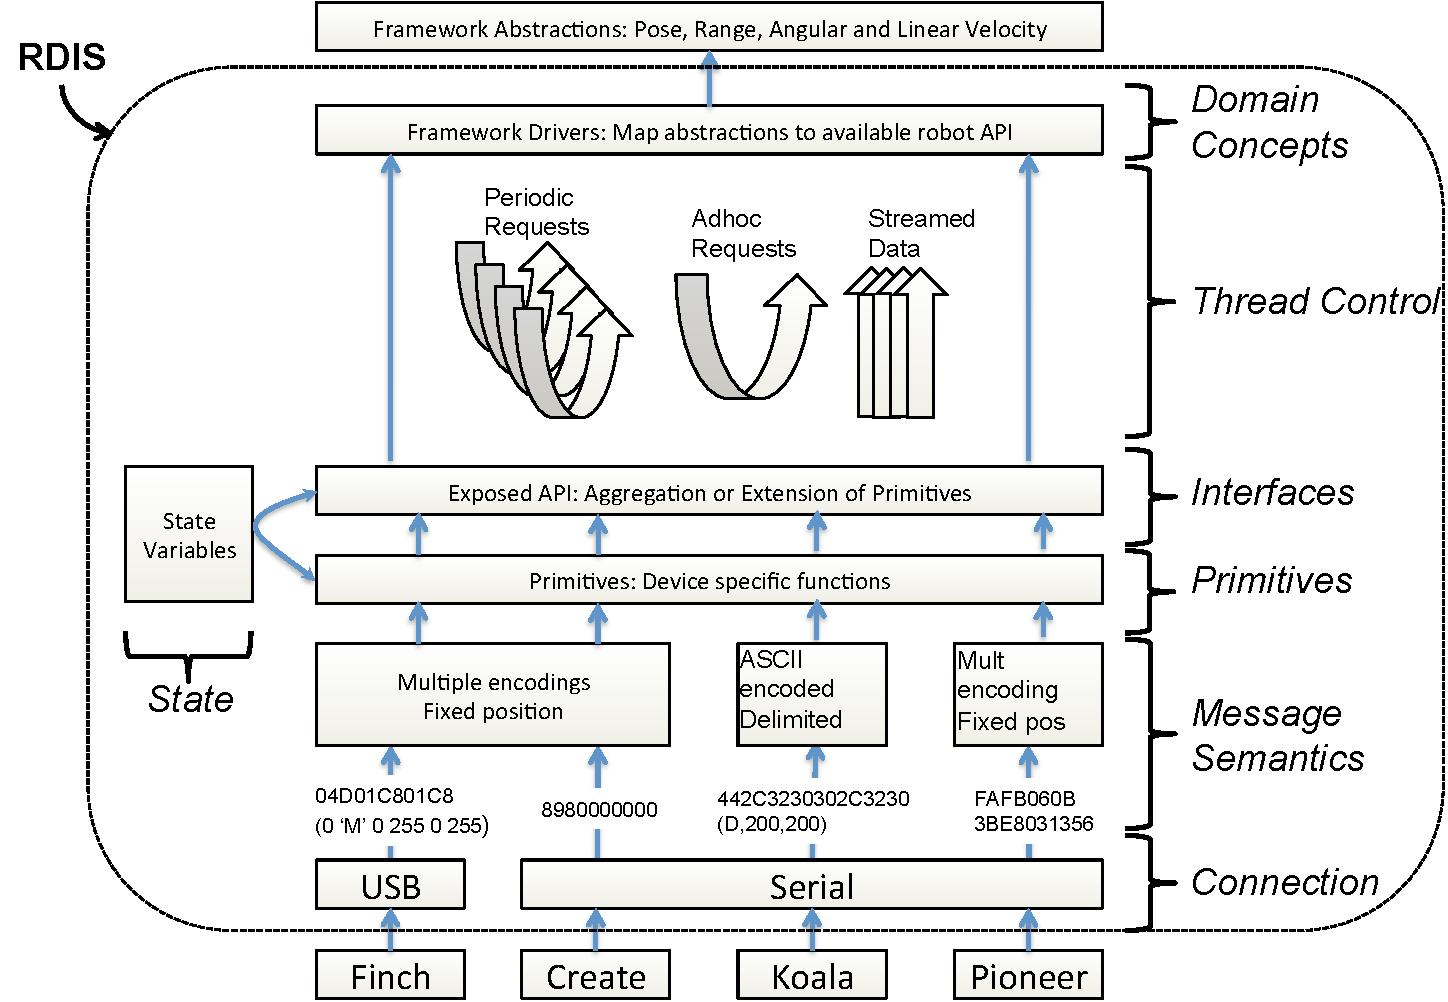
\includegraphics[width=6in]{images/dm.pdf}
      \caption{Preliminary domain model for mapping devices to frameworks \cite{Anderson2012}.}
      \label{dm}
\end{figure*}

The preliminary result supports the idea that general robot devices can be described declaratively in a manner that supports discovery and that links to the back-end processes.  RDIS must be expanded to be useful for a larger pool for robot platforms and frameworks.  The work proposed as part of this effort will accomplish the following major innovations to RDIS as a contribution to the engineering of cyber-physical systems: 
\begin{enumerate}
\item Extend the actuation model to include a larger set of popular kinematic chains from both manufacturing and exploration robotics, and
\item Extend the processing models to include a larger set of execution semantics, 
\item Create a supporting set of tools and frameworks that supports prototyping, evaluation and adoption.   
\end{enumerate}

\subsection{Expansion of domain concepts to additional kinematic chains}
\label{sec:kin}

\begin{figure*}[thpb]
      \centering
      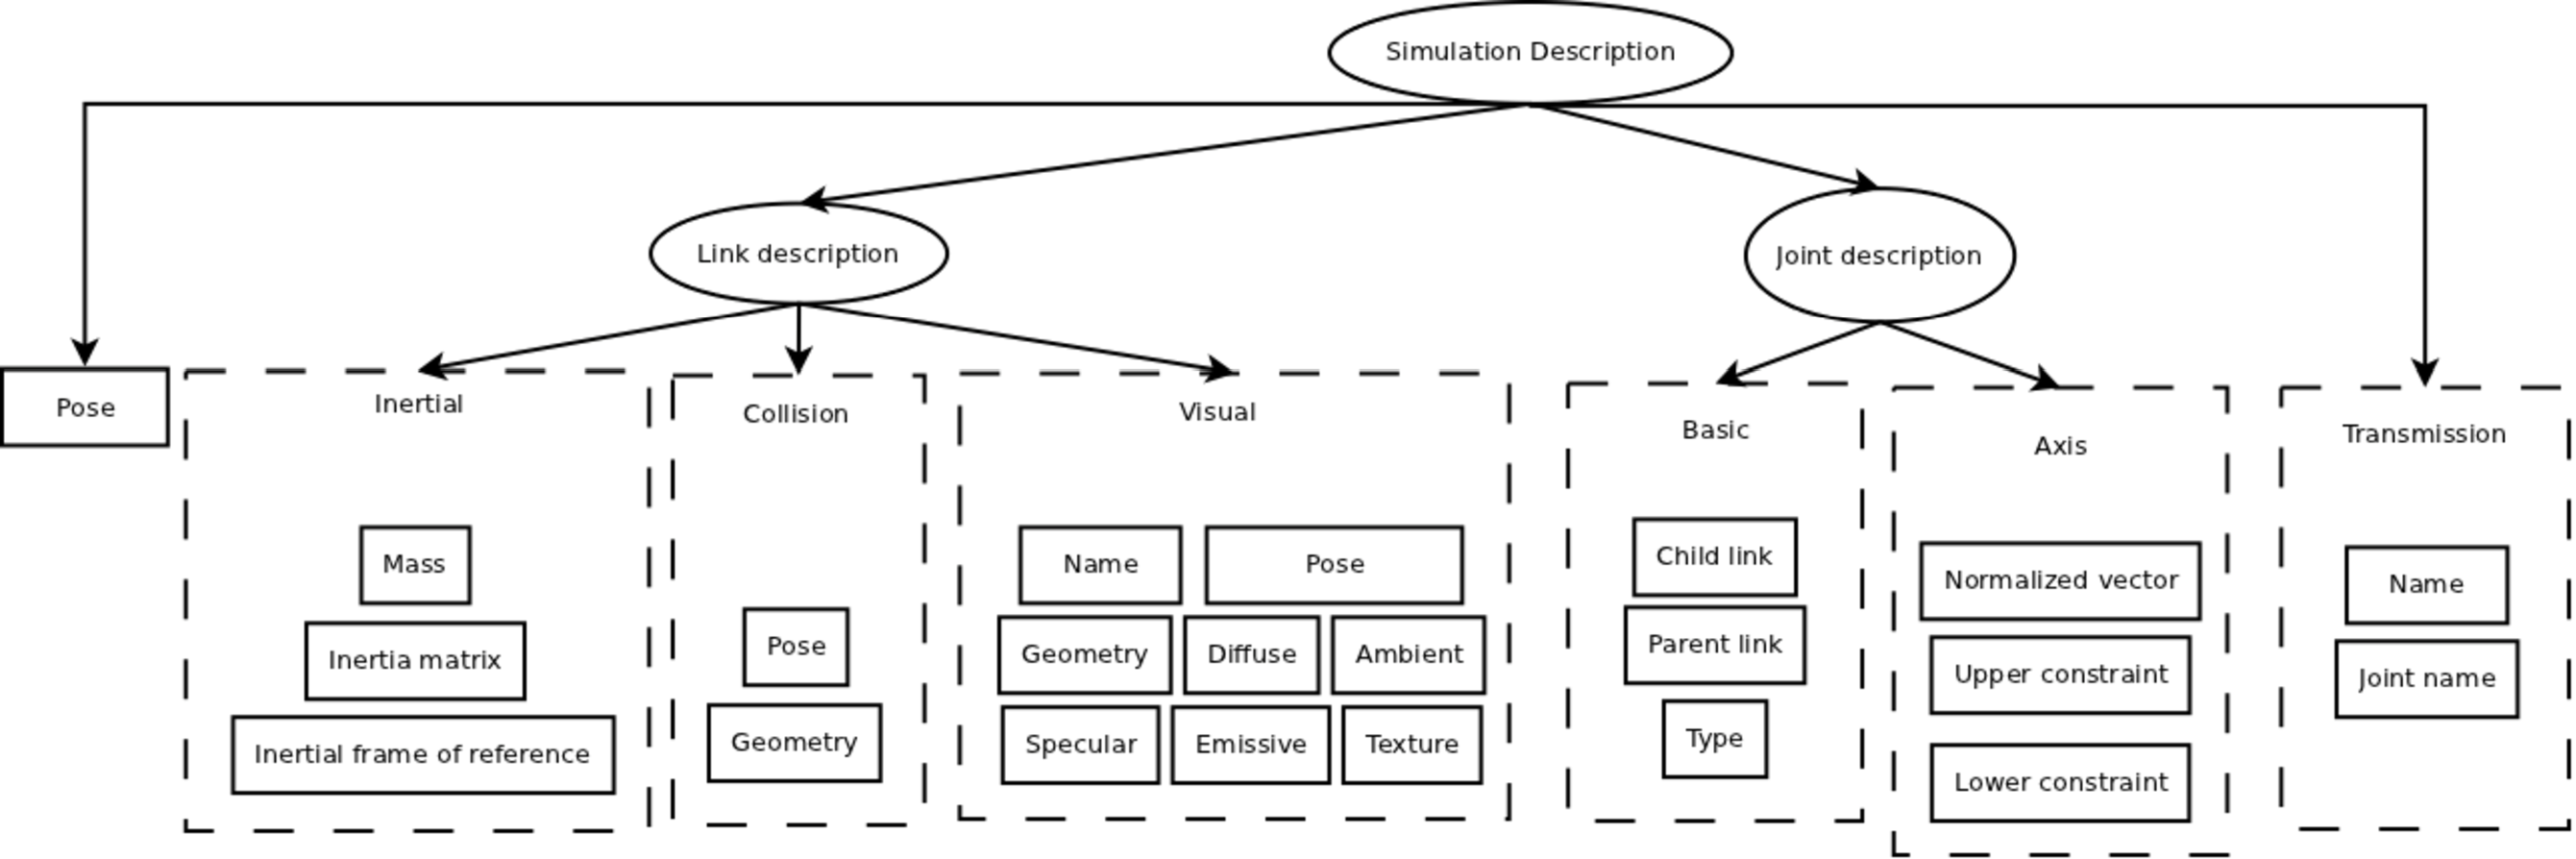
\includegraphics[width=6in]{images/kvc.pdf}
      \caption{General model for describing kinematics, appearance, collision and dynamics parameters sufficient for simulation.  Currently targeted platforms include Gazebo, Webots, and ROS.}
      \label{kvc}
\end{figure*}

Domain concepts map interfaces to domain-specific concepts in a framework agnostic manner.  Each framework has a notion of a general set of abstract data types generated from device drivers such as pose estimates, pose relative to an identified landmark, control via linear and angular velocity along a dimension or axis, and point and fields of open distance.  The {\sc Domain concepts} definition identifies interfaces that map to the abstract concepts allowing for templates to map the abstract concepts to the existing interfaces available on a device.

From the previous sections it is apparent that the robot kinematic modeling languages are missing necessary components for a generalized description for use in simulation. Some description formats do well in defining the geometries of the robot, but make categorical assumptions about the kinematics of the robot, offloading the actual kinematic description to the framework itself. As an example, Stage has a drive ``diff'' statement to label a position element as having differential-drive steering, and Webots has a DifferentialWheels node which acts as the base node of a robot description having differential steering. URDF solves this by defining a relationship between transmissions and joints, but its approach is specific to the PR2 robot.

Current models of kinematics are adept at modeling the construction of the robot in a way that is almost a standard. However, what is missing between all of them is how to model controllable joints. If a solid mapping can be defined between programming interfaces and resultant efforts at joints, this would benefit the robotics community greatly as there is not currently a description format which does so without the aid of a companion plugin or hardware description. RDIS would benefit much from this component as well as it would define the bridge between the control model introduced in earlier work \cite{Anderson2012} and the kinematic model which it currently lacks. Thus, the work that needs to be done is to define RDIS's kinematic model according to the trends seen from other frameworks and then provide a mapping from interfaces in the control model to transmission efforts at joints in the kinematic model. It is clear that a viable robot kinematic model will somehow take heed of some of the existing description formats to ensure there is sufficient compatibility with the model. The problem lies in deciding which parameters are essential to a proper kinematic modeling and which are parameters which lose meaning when carried to other frameworks. An additional goal is to find a concise set of these parameters such that no one parameter may be defined in terms of other parameters. 

Figure \ref{kvc} details the concepts in the updated working model for expanded kinematics.  LINK and JOINT are composed from similar concepts in existing frameworks and simulation descriptions.  The LINK is an atomic rigid body in the robot's structure which constitutes the majority of the robot's composure by mass. A link is a primary parameter to the physics simulation as it contains the parameters necessary to simulate the physics of a robot. Additionally, a simulator typically has a visual representation of the robot to present to the user and a LINK will represent the majority of the visualization, so there will be parameters which are to be used by the simulation renderer. Finally, as the LINK is the only material component in the robot model, it will serve as the basis for the collision model, so the parameters to the collision engine must also be defined.

The JOINT component of the model characterizes a set of constraints imposed on two joints. In this relationship, there is strictly one related parent LINK and one child LINK. There are six degrees of freedom between two unconstrained links, and a joint restrains one or many of them. The standard degrees of freedom are X, Y, Z, roll, pitch, and yaw. From the examined frameworks, three main types of joints reappear between frameworks, all of which JOINT generalizes a prismatic joint constrains all degrees of freedom except for Z. This allows child link to translate freely in one dimension with respect to the parent link's frame. By convention, this is normally the Z-axis in joint space. This type of joint might be used to model a gripper for a robot arm.
%
A hinge joint constrains all degrees of freedom except for pitch. This allows a link to rotate in one dimension about a single point of rotation with respect to its parent link's frame. This type of joint might be used to model a fixed wheel on a differential drive robot if no bounds were posed on the joint rotation.  A ball-and-socket joint constrains X, Y, and Z. This allows for rotation of a link about any of its axes with respect to its parent link. This type of joint might be used to model a spherical caster wheel for a differential drive robot.

%Because of the strength of the model, LINK and JOINT have already been examined extensively from many different viewpoints, resulting in a mature description of each of these components in just URDF or SDF. It is the PIs' opinion that these components are described well by these formats and there is not much to discover save for minute details. 

%\subsubsection{Link}
%The LINK is an atomic rigid body in the robot's structure which constitutes the majority of the robot's composure by mass. A link is a primary parameter to the physics simulation as it contains the parameters necessary to simulate the physics of a robot. Additionally, a simulator typically has a visual representation of the robot to present to the user and a LINK will represent the majority of the visualization, so there will be parameters which are to be used by the simulation renderer. Finally, as the LINK is the only material component in the robot model, it will serve as the basis for the collision model, so the parameters to the collision engine must also be defined.
%
%\begin{enumerate}
%\item The {\sc physics} component of the description of LINK defines the parameters needed for physics simulation. This will include the robot mass, rotational inertia matrix, and the inertial frame of reference. This portion of the model is consistent in frameworks which simulate the dynamics of robots. SDF introduces a linear and angular velocity damping in this component, however it was alone in this specification. As the implementation proceeds, it will be apparent if this component is missing any parameters.
%
%\item The {\sc collision} component describes the parameters needed by the collision engine. Generally in most simulation description formats, the main components were the pose of the collision model and the simple geometry which defines it. This is to be differentiated from the visual geometry, as it is not necessarily true that a collision geometry may be used as a visual geometry or vice-versa. For instance, Webots uses an IndexedFaceSet type to represent complex or high-fidelity geometries for the visual component of a robot, however this complex type of geometry would be a strain for the collision engine so it is not available for use as a collision geometry. A challenge in defining this component is deciding which collision geometries will effectively represent most robots. 
%
%\item The {\sc visual} component describes the parameters provided to the scene rendering engine. Visual representations are most easily characterized by some sort of geometry, which tended to be the observed pattern within most simulation frameworks. It should be noted that not all frameworks separate the collision model and the visual model. In this case, it usually marks that the simulator is simplistic and does not provide a high definition visual representation of the simulation. In these cases, one geometry is defined to serve as both the collision and visual geometry. In the context of our model, the collision geometry should be selected as it is assumed to be the most simplistic. Solving the collision geometry problem should also determine at least a subset of visual geometries. An additional challenge to defining the visual component will be handling mesh types. Between Webots and Gazebo, there are mesh types ranging from the standard triangle mesh to polygon meshes to height maps. As well, if meshes are supported they are best referenced as they will cloud the description file. 
%\end{enumerate}
%
%\subsubsection{Joint} 
%The JOINT component of the model characterizes a set of constraints imposed on two joints. In this relationship, there is strictly one related parent LINK and one child LINK. There are six degrees of freedom between two unconstrained links, and a joint restrains one or many of them. The standard degrees of freedom are X, Y, Z, roll, pitch, and yaw. From the examined frameworks, three main types of joints reappear between frameworks, all of which JOINT generalizes a prismatic joint constrains all degrees of freedom except for Z. This allows child link to translate freely in one dimension with respect to the parent link's frame. By convention, this is normally the Z-axis in joint space. This type of joint might be used to model a gripper for a robot arm.
%
%A hinge joint constrains all degrees of freedom except for pitch. This allows a link to rotate in one dimension about a single point of rotation with respect to its parent link's frame. This type of joint might be used to model a fixed wheel on a differential drive robot if no bounds were posed on the joint rotation.  A ball-and-socket joint constrains X, Y, and Z. This allows for rotation of a link about any of its axes with respect to its parent link. This type of joint might be used to model a spherical caster wheel for a differential drive robot.


A TRANSMISSION component is not yet well-defined in the current state-of-the-art in robot modeling, therefore it may contain some parameters which are to be discovered. From the previously discussed frameworks, URDF was the only description format which included this component, which the documentation notes was not intended to be used for anything but the PR2 robot. Generally speaking, it is known that a transmission is supposed to define how a motor applies effort to a joint or several joints. Therefore, it can be concluded that a transmission must have an association with at least one joint.

Additionally, transmissions mark a point of control for the robot application. If an application wishes to command a robot to move in some manner, then the application must utilize the appropriate interfaces, which in turn triggers one or more robot control primitives which alter the state of the joints. Therefore, a primitive must somehow relate to some transmission and subsequently the parameters provided to the primitive. For example, it could be possible to translate a motor speed to the effort applied at that joint declaratively, and this might require a modification to the previously mentioned control model at the PRIMITIVE component. 

With the major components of the model identified via a survey of existing frameworks, what remains is to discover which components are required to produce a full implementation of the RDIS model. To that end, further research is required. At this point, the relationship between the kinematic model and the control model have been established. The specifics of what is contained in the kinematic and control packages is within the scope of this project. The control model is expected to change slightly to provide support for manipulation of the kinematic model during simulation, while the kinematic model will be wholly new to RDIS while the bindings between the control model and the kinematic model will be clearly defined as a contribution to the robotics modeling community.

\subsection{Expansion of execution semantics}

The ability to generalize device to framework mapping requires documenting the concepts in existing mappings.  The domain model captures the invariant features of the device to framework mapping drives the contents of RDIS.  In Figure \ref{dm}, the domain is broken into seven related concepts: connections, state, message semantics, primitives, interfaces, thread control, and robotics domain concepts.  {\sc Connection} refers to the transport used to communicate from the device driver to the framework.  Information needed to establish and maintain the connection is defined within this concept. The {\sc State} definition serves two purposes: 1) define constants relevant to other sections and 2) allow for state to be saved and retrieved as part of adhoc and periodic requests.   The {\sc Message Semantics} refers to the structure of the data which is actually sent to the robot over the connection. This specification is decided by the manufacturer and is generally uniform between primitives.   {\sc Primitives} focus on describing the firmware interface in order to document the invariant features of the device.   The {\sc Interface} declaration, acting as a logical view of the {\sc Primitives},  specifies functions that are available to a developer to control a robot.   {\sc Domain Concepts} map interfaces to domain specific concepts in a framework agnostic manner.  These concepts are discussed in detail in \cite{Anderson2012}.



%These changes require updates to the specification and the underlying set of generation and utilizing tools. 

In this research, we expand the basic implementation of each concept to accommodate a larger set of embedded firmware controllers.  These tasks include: 
\begin{enumerate}
\item Addition of a complete kinematic, visual and collision description consistent with existing simulators and frameworks (see Figure \ref{kvc}).  The proposed model is designed to accommodate other kinematic chains used for manufacturing and mobile manipulation (discussed in Section \ref{sec:kin}). 
\item Standard mechanism for error handling and notification at both the communication and primitive levels.  Error handling examples include re-establishment of connection or actions to take based on output parameters.  This is particularly relevant to platforms that require a heartbeat request periodically.
\item Expansion of the initial single-threaded implementation to include dual and multi-threading models.  A dual model accommodates different input and output threads while a multithreaded model support different frequencies for periodically submitted requests. 
\item Refinement of the state concept and how it matches to primitives and interfaces would provide a scripting language for transformation of data.  The state variable concept is instrumental in implementing periodic requests asynchronously from the client request/reply system.
\item Management of sensor and actuator error models consistent with existing frameworks will allow for manufacturer provided error models to be propagated to the framework or controller.  An example would be a transformation of encoder error to pose error.  Although all sources of error (systematic and non-systematic) cannot be accounted for in this approach, it is currently better than existing approaches that abstract out specific device errors.
\end{enumerate}



\subsection{Prototyping, Evaluation and Adoption: RDIS-enabled Tools and Frameworks}

This challenge focuses on assisting the developer in defining framework drivers that enable the communication with individual devices.
We propose a modeling approach where the definitions and mappings are specified independently from the actual framework (\eg ROS, Player) and robot (\eg Create, Pioneer).
This is achieved by defining RDIS as a DSL rather than using general purpose languages to reduce technical and accidental complexity~\cite{Brooks1987}.
Domain-specific modeling~\cite{Kelly2008}, and in general model-driven engineering (MDE~\cite{Stahl2006}), is an approach that allows models to be manipulated at the level of abstraction of the application domain the model is intended for, rather than at the level of computing.
To bridge the gap between the application domain and the solution domain, MDE uses models to describe complex systems at multiple levels of abstraction and through automated support for transforming and analyzing models.
A DSL is defined by means of a \emph{meta-model} that represents the key abstractions and intentions of an expert in a particular domain (in our case frameworks and robotic devices).
A meta-model thus specifies the abstract syntax and static semantics of the set of model instances of that language.
A model represents an abstraction of the real system, capturing some of its essential properties in order to simulate, and generate code for applications.
The manipulation of models is performed through the use of \emph{model transformation}.
It transforms a source model into a target model, both conforming to their respective meta-model.
Although a model transformation is defined at the meta-model level, it is applied and executed on models.

In order to map the messages exchanges between arbitrary frameworks and robots, RDIS will comprise two meta-models.
The first one abstracts the concepts from frameworks.
We have already developed a prototype of the models as part of a student project in an advanced graduate course that PI Syriani teaches.
The framework meta-model is currently based on reverse-engineering ROS (still in early stages).
We plan to perform the same task for the different frameworks to be able to define a framework-independent meta-model.
Similarly, we will investigate how this can be performed on the devices side.

Once the meta-models of the language are defined, a rule-based model transformation specify the mapping between them~\cite{Jouault2008}.
A rule is a declarative construct that dictates ``what'' shall be transformed and not ``how''.
It consists of pre-condition and post-condition patterns~\cite{Ehrig2006}.
The pre-condition pattern determines the applicability of a rule: it is usually described with a left-hand side (LHS) and optional negative application conditions (NACs).
The LHS defines the pattern that must be found in the input model to apply the rule.
The NAC defines a pattern that shall not be present, inhibiting the application of the rule.
The right-hand side (RHS) imposes the post-condition pattern to be found after the rule was applied.
An advantage of using the rule-based transformation paradigm is that it allows to specify the transformation as a set of operational rewriting rules instead of using imperative programming languages.
Model transformation can thus be specified at a higher level of abstraction (hiding the implementation of the matching algorithms and the modifications of the data structures), closer to the domain of the models the transformation is applied to.
Code generators will also be implemented from the RDIS meta-models to each platform in order to deploy the hardware.

The evaluation of RDIS and the developed models will be conducted following these criteria:
\vspace{-.5\baselineskip}%
\begin{itemize}
  \item RDIS should be extended to be a model which contains the association between the exposed control interfaces and the behavior which is actuated in
  simulation.
  \item RDIS should be general enough to model more than one kinematic category of robot and more than one robot within a category of kinematic design.
  \item RDIS should be descriptive enough so that the model is rigorously simulatable.
  \item There should be a mapping between the components and their associations from RDIS to at least one of the major simulation descriptions (Stage, URDF, SDF, and Webots are worthy targets).
  \item RDIS is concise (not redundant) as measured via model metrics.
  \item RDIS generated development modules should be sufficiently easy to use as evaluated based on user study and evaluation.
\end{itemize}

This research will generate a set of artifacts and tools to support the prototyping and evaluation of the domain model and its accompanying language specification.  These artifacts encompass three categories: 1) Language definition through language parsers and generators, 2) Framework and language bridge tools and 3) Model metrics and evaluation artifacts.  The existing grammar for RDIS will be updated and maintained in a open SVN repository as well as publicized in the CPS Virtual Organization (see Data Management Plan).\newline



\section{Curriculum Development Activities}\label{sec:curriculum}

Education, courses



\section{Schedule}\label{sec:schedule}

Tasks and timeline.



\section{Results from Prior NSF Support}\label{sec:prior-nsf}
\begin{enumerate}
\item Monica Anderson  - PI for the NSF Grant: CCLI: Enhancing student motivation in the first year computing science curriculum (DUE- 0736789), 04/01/2008-08/31/2011.  This is an ongoing project that addresses retention issues due to motivation through specially designed modules that use PREOP in a CS0 or CS1 laboratory setting.  We provided PREOP workshops to teachers at the ARTSI Faculty Meeting, demonstrated PREOP at the Google education summit and added PREOP to Alice instructor training (July 2011). Three papers have been published including two conference papers and two journal papers \cite{Davis2009,wellman2009alice,Wellman2009b,Anderson}. 
\item Monica Anderson  - PI for the Grant: ARTSI-Advancing Robotic Technology for Societal Impact (BPC-A- 0742123), 09/01/07-12/31/2012. This is an ongoing broadening participation grant that increases the number of students interested in computer science and robotics through both research and creative experiences. Robotics programs have been established or enhanced at 14 HBCUs. The PI has provided each school with both onsite and remote instructional support ranging from hands-on workshops on open-source robotics development environments and controller development to hardware assembly instructions. Seven summer research assistants have been hosted at UA, with one student contributing to an accepted paper \cite{Wellman2009} and resulting in numerous poster presentations. 
\item Monica Anderson  - PI for the Grant: SGER: Impact of Intermittent Networks on Team-based Coverage (IIS-0846976), 09/01/2008-08/31/2009. This project investigated both surveillance in constrained environments using limited resources and methods for coordinating robot teams with limited communications capability. The novel approach of using ALUL and a QOS metric allowed for balanced target acquisition and tracking \cite{Veluchamy2010,Alexander2009,Mckenzie2010,McKenzie2009}.
\item Monica Anderson  - Co-PI for the Grant: EMT: Collaborative Research: Primate-inspired Heterogeneous Mobile and Static Sensor Networks (CNS: 0829827) 09/01/2008-08/31/2011. This project investigates bio-inspired approaches for multirobot coordination. We show that given a greedy approach to selecting the next point to search, observation information provides more relevant input to the next action selected. Experimental results show that using observation to infer state and intent to disperse nodes performs better than non-communicative and potential field based cooperation and in some cases direct communications. \cite{Wellman2009d,Dawson2011,Dawson2010,Dawson2011b,Wellman2009c}. 
\item Monica Anderson  - PI for the Grant: University of Alabama Participation of EPSCOR Institution in SSR-RC: QOS service metrics for unmanned surveillance (IIP: 1026528).  06/15/2010-06/14/2012. We consider ALUL as a metric that indicates the target acquisition ability of a particular system configuration. When used in conjunction with temporal constraints, we can intelligently automate camera coverage to improve target acquisition and tracking performance of the system. The results from the experiments confirm that the coverage in constrained environments when the existing camera configuration cannot view large portions of the region of our interest improves when ALUL is considered.  To date, one conference paper and one journal article have been accepted \cite{Veluchamy2011,Dukeman2011}.
\item Eugene Syriani - new investigator and has no prior NSF support.

\end{enumerate}


\clearpage
\setcounter{page}{1}

%%%%%%%%%%%%%%%%%%%%%%%%%%%%%%%%%%%%%%%%%%%%%%%%%%%%%%%%%%%%%%%%%%%

% Specify the bibliography style and data
\bibliographystyle{cj}
%\bibliography{bibliography}

\clearpage


\section*{Data Management Plan}


\subsection*{Types of data produced by this project include:}

Source code artifacts include: 1)source code for programs that create, validate and use the RDIS data, 2) grammars and programs that will be used to generate source code for creating, validating and using the RDIS data, 3) source code for framework integration including ROS nodes, packages and stacks, 4) source code for eclipse plug ins, and 5) sample programs, documentation and build files.  Curriculum modules include those created for the domain modeling and robotics courses.  Human Subject Identifiable Data include completed surveys and interview notes and logs gathered from user studies of RDIS and RDIS-enabled tools 

\subsection*{Standards to be used for data and metadata format and content }

\subsubsection*{Source Code:}  The practice of making code available via source code repository is deemed sufficient.  Standard file naming, organization and coding style practices will apply based on the language and platform being targeted.

\subsubsection*{Curriculum: } Documents will be made available in PDF, Word or Latex formats.

\subsubsection*{ Human Subject Identifiable Data:}Survey instruments and interview questions will be made available as part of publications.

\subsection*{Policies for Access and sharing}

\subsubsection*{Source Code:} Source code will be available via publicly accessible, web-enabled source control as its results are published.  

\subsubsection*{Curriculum:} Curriculum modules will be available on the project website.

\subsubsection*{Human Subject Identifiable Data:} Since the data will be from human subjects, appropriate protocols will be instituted to protect individual's privacy. Evaluation activities will be approved by the University of Alabama Institutional Review Board. Confidentiality of participant information will be placed as a high priority in all evaluation activities. Hence, data accessible to the project and to other researchers will not be identifiable with an individual. All data will be stored using code number identifiers in encrypted files. Access to files will be through passwords provided to appropriate project staff. Data will be stored in locked filed cabinets in a secure site and on portable hard drives by dedicated university encrypted computers at a secure location readily accessible to the project PI and personnel. Raw data will be accessible only to appropriate project staff designated by the PI.

\subsection*{Policies for Re-Use}

\subsubsection*{Source code and curriculum materials:} We will release all software artifacts developed in association with this project under the \textit{BSD 3-Clause License} (the ``New BSD'' license) and will make them available via an appropriate outlet such as Google Project Hosting.


\subsubsection*{Human subject data} Human subject data will only be available in aggregated form for the protection of the participants.  Detailed aggregate findings will be available as technical reports and will also be published.

\subsection*{Plans for Archiving Data and for Preservation of Access}
\subsubsection*{Personally identifiable data} Personally identifiable data will be stored in locked file cabinets in a secure site and on portable hard drives by dedicated encrypted computers for 9 years from the beginning of the project and destroyed in a secure manner at the end of that period. Raw data will be accessible only to appropriate project staff designated by the PI. Long term access will be available from secure storage at the University of Alabama upon agreement to a written request sent to the project PI or, if the PI is not available, to the University of Alabama's Office of Sponsored Programs. Payment to the university of costs incurred for the copying and delivery of data will be required.

\subsection*{Other Notes:}

We will publish our results in leading conferences and journals as well as make results and methodologies available via the CPS Virtual Organization (PI is already a member). As is typical in the software engineering community, we will rigorously define our experimental procedures. For example, for each case study we will provide the definition and context, including subject software systems, benchmarks, metrics, and the study setting. In addition, we will document our research questions and hypotheses, our data collection and analysis procedures, results, and threats to validity. We will provide access to our data files via online appendices.  We will distribute annual reports via our web site.


\end{document}
